% Author: Victor Terron (c) 2014
% Email: `echo vt2rron1iaa32s | tr 132 @.e`
% License: GNU GPLv3

\documentclass[14pt]{beamer}

\usepackage[utf8]{inputenc}
\usepackage{listings}

\usepackage{minted}
\usemintedstyle{emacs} % of course

% Set global options for \inputminted
% https://tex.stackexchange.com/a/103191/48441
\newmintedfile[pythoncode]{python}{
  fontfamily=tt,
  linenos=true,
  numberblanklines=true,
  numbersep=12pt,
  numbersep=5pt,
  gobble=0,
  frame=leftline,
  framerule=0.4pt,
  framesep=2mm,
  funcnamehighlighting=true,
  tabsize=4,
  obeytabs=false,
  mathescape=false
  samepage=false,
  showspaces=false,
  showtabs =false,
  texcl=false,
}

% Enable accents and ñ in our code listings
% http://stackoverflow.com/a/2782147/184363
\lstset{
  literate={á}{{\'a}}1
           {é}{{\'e}}1
           {í}{{\'i}}1
           {ó}{{\'o}}1
           {ú}{{\'u}}1
           {ñ}{{\~n}}1
           {¡}{{\textexclamdown}}1
}

\usetheme{Copenhagen}
\useoutertheme{infolines}
\setbeamercovered{dynamic}

\title{Clases en Python: lo estás haciendo mal}
\author{Víctor Terrón}
\date{9 de noviembre de 2014}
\institute{IAA-CSIC}

\begin{document}

\section{Introducción}
% Author: Victor Terron (c) 2014
% Email: `echo vt2rron1iaa32s | tr 132 @.e`
% License: CC BY-SA 4.0

\begin{frame}{Programación orientada a objetos}
  \small
  \begin{block}
    {\centering Una cita apócrifa}
    \centering
    ``Object-oriented programming is an exceptionally bad
    idea which could only have originated in California''
    [Edsger W. Dijkstra]
  \end{block}

  \begin{figure}
    \centering
    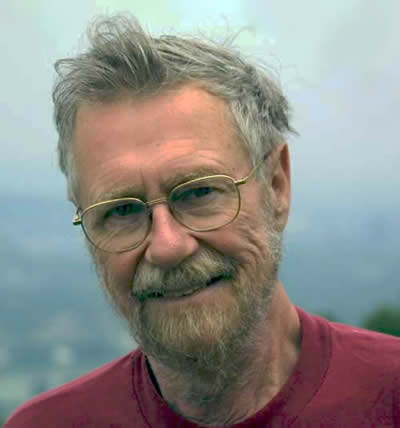
\includegraphics[height=4cm]{pics/dijkstra.jpg}
  \end{figure}
\end{frame}

\begin{frame}{Programación orientada a objetos}
  \small
  \begin{block}
    {\centering Lo que en realidad dijo}
    \centering
    ``For those who have wondered: I don't think object-oriented
    programming is a structuring paradigm that meets my standards of
    elegance.'' [Edsger W. Dijkstra, 1999]
    [\href{http://www.cs.utexas.edu/users/EWD/transcriptions/EWD12xx/EWD1284.html}
      {\structure{Fuente}}]
  \end{block}

  \begin{figure}
    \centering
    
\includegraphics[height=5cm]{pics/like-a-sir.png}
  \end{figure}
\end{frame}

\begin{frame}{Programando clases en Python}
  \begin{block}{}
    \Large
    \centering
    El objetivo de esta charla es ayudarnos a hacer
    \structure{idiomáticas} y \structure{elegantes} nuestras clases en
    Python.
  \end{block}

  \begin{justify}
    En mayor o menor medida todo el mundo usa programación orientada a
    objetos, pero hay una serie de aspectos fundamentales que es
    indispensable conocer para evitar que nuestro código sea
    innecesariamente feo o complejo.
  \end{justify}
\end{frame}

\begin{frame}{Nuestra reacción a veces}
  \begin{figure}
    \centering
    
\includegraphics[height=6cm]{pics/dont-want-to-live-on-this-planet.png}
  \end{figure}
\end{frame}

\begin{frame}{Programando clases en Python}
  \begin{alertblock}{}
    \small
    \centering
    La premisa es que somos mínimamente familiares con los
    \structure{conceptos básicos} de programación orientada a objetos,
    y que hemos trabajado un poco con nuestras propias clases en
    Python.
  \end{alertblock}

  \begin{figure}
    \centering
    
\includegraphics[height=4cm]{pics/captain-obvious.jpg}
  \end{figure}
\end{frame}

\begin{frame}{Un muy brevísimo repaso}
  \begin{itemize}
    \item Llamamos \structure{clase} a la representación abstracta de un
      concepto. Por ejemplo, 'perro', 'número entero' o 'servidor web'.
    \item Las clases se componen de \structure{atributos} y
      \structure{métodos}.
    \item Un objeto es cada una de las instancias de una clase.
  \end{itemize}
\end{frame}

\begin{frame}{Ejemplo: clase Perro}
  \pythoncode[fontsize=\footnotesize]{intro.py}
\end{frame}

\begin{frame}{¡No os limitéis a escuchar!}
  \begin{center}
    No suele ser divertido escuchar a nadie hablar durante casi una
    hora. Participad, intervenid, criticad, opinad. ¡Si digo algo que
    no tiene ningún sentido, \structure{corregidme}!
  \end{center}

  \begin{block}{\centering El código fuente está disponible en:}
    \centering \url{http://github.com/vterron/PyConES-2014}
  \end{block}

  \begin{center}
    \small Erratas, correcciones, enlaces, ¡cualquier cosa!
  \end{center}
\end{frame}


\end{document}

